\documentclass[xcolor=dvipsnames,notes]{beamer}
\usecolortheme[named=Brown]{structure}
\usetheme{default}
\setbeamertemplate{navigation symbols}{} 
\usepackage{tikz}
\usetikzlibrary{arrows,decorations.pathmorphing,backgrounds,positioning,fit}
\usetikzlibrary{datavisualization.formats.functions}
\usetikzlibrary{shapes}
%     
%Here are some macro's saving time and labour:     
%     
\newcommand{\const}{\mbox{const}}      
\newcommand{\est}{\mbox{{\tiny est}}}      
\newcommand{\im}{\mbox{$\Im \mbox{m}$}}      
\newcommand{\obs}{\mbox{{\tiny obs}}}      
\newcommand{\otherwise}{\mbox{otherwise}}      
\newcommand{\real}{\mbox{$\Re \mbox{e}$}}      
\newcommand{\sign}{\mbox{sign}}      
\newcommand{\sinc}{\mbox{sinc}}      
%
\newcommand{\p}{\mbox{$\partial$}}      
\renewcommand{\d}{\mbox{$\partial$}}      
\newcommand{\w}{\mbox{$\omega$}}      
%
\newcommand{\AAA}{\mbox{\boldmath $A$}}   
\newcommand{\BB}{\mbox{\boldmath $B$}}     
\newcommand{\CC}{\mbox{\boldmath $C$}}     
\newcommand{\DD}{\mbox{\boldmath $D$}}     
\newcommand{\EE}{\mbox{\boldmath $E$}}     
\newcommand{\FF}{\mbox{\boldmath $F$}}   
\newcommand{\GG}{\mbox{\boldmath $G$}}   
\newcommand{\HH}{\mbox{\boldmath $H$}}   
\newcommand{\II}{\mbox{\boldmath $I$}}   
\newcommand{\JJ}{\mbox{\boldmath $J$}}   
\newcommand{\KK}{\mbox{\boldmath $K$}}   
\newcommand{\LL}{\mbox{\boldmath $L$}}   
\newcommand{\MM}{\mbox{\boldmath $M$}}   
\newcommand{\NN}{\mbox{\boldmath $N$}}   
\newcommand{\OO}{\mbox{\boldmath $O$}}   
\newcommand{\PP}{\mbox{\boldmath $P$}}   
\newcommand{\QQ}{\mbox{\boldmath $Q$}}   
\newcommand{\RR}{\mbox{\boldmath $R$}}   
\newcommand{\SSS}{\mbox{\boldmath $S$}}   
\newcommand{\TT}{\mbox{\boldmath $T$}}   
\newcommand{\UU}{\mbox{\boldmath $U$}}   
\newcommand{\VV}{\mbox{\boldmath $V$}}   
\newcommand{\WW}{\mbox{\boldmath $W$}}   
\newcommand{\XX}{\mbox{\boldmath $X$}}   
\newcommand{\YY}{\mbox{\boldmath $Y$}}   
\newcommand{\ZZ}{\mbox{\boldmath $Z$}}   
%
%\newcommand{\aaa}{\mbox{\boldmath $a$}}     
\newcommand{\bb}{\mbox{\boldmath $b$}}     
\newcommand{\cc}{\mbox{\boldmath $c$}}     
\newcommand{\dd}{\mbox{\boldmath $d$}}     
\newcommand{\ee}{\mbox{\boldmath $e$}}   
\newcommand{\ff}{\mbox{\boldmath $f$}}   
%\newcommand{\ggg}{\mbox{\boldmath $g$}}   
\newcommand{\hh}{\mbox{\boldmath $h$}}   
\newcommand{\ii}{\mbox{\boldmath $i$}}   
\newcommand{\jj}{\mbox{\boldmath $j$}}   
\newcommand{\kk}{\mbox{\boldmath $k$}}   
%\newcommand{\lll}{\mbox{\boldmath $l$}}   
\newcommand{\mm}{\mbox{\boldmath $m$}}   
\newcommand{\nn}{\mbox{\boldmath $n$}}   
\newcommand{\pp}{\mbox{\boldmath $p$}}   
\newcommand{\qq}{\mbox{\boldmath $q$}}   
\newcommand{\rr}{\mbox{\boldmath $r$}}   
%\newcommand{\sss}{\mbox{\boldmath $s$}}   
%\newcommand{\ttt}{\mbox{\boldmath $t$}}   
\newcommand{\uu}{\mbox{\boldmath $u$}}   
\newcommand{\vv}{\mbox{\boldmath $v$}}   
\newcommand{\ww}{\mbox{\boldmath $w$}}   
\newcommand{\xx}{\mbox{\boldmath $x$}}   
\newcommand{\yy}{\mbox{\boldmath $y$}}   
\newcommand{\zz}{\mbox{\boldmath $z$}}   
%
\newcommand{\balpha}{\mbox{\boldmath $\alpha$}}     
\newcommand{\bpsi}{\mbox{\boldmath $\psi$}}     
\newcommand{\bphi}{\mbox{\boldmath $\phi$}}     
\newcommand{\bbeta}{\mbox{\boldmath $\beta$}}     
\newcommand{\btheta}{\mbox{\boldmath $\theta$}}     
\newcommand{\bdelta}{\mbox{\boldmath $\delta$}}     
\newcommand{\bgamma}{\mbox{\boldmath $d$}}     
\newcommand{\bGamma}{\mbox{\boldmath $\Gamma$}}     
\newcommand{\bLambda}{\mbox{\boldmath $\Lambda$}}     
\newcommand{\bmu}{\mbox{\boldmath $\mu$}}     
\newcommand{\bnabla}{\mbox{\boldmath $\nabla$}}     
\newcommand{\brho}{\mbox{\boldmath $\rho$}}     
\newcommand{\bSigma}{\mbox{\boldmath $\Sigma$}}     
\newcommand{\bsigma}{\mbox{\boldmath $\sigma$}}     
\newcommand{\bxi}{\mbox{\boldmath $\xi$}}     
\newcommand{\bepsilon}{\mbox{\boldmath $\epsilon$}}     
\newcommand{\blambda}{\mbox{\boldmath $\lambda$}}     
\newcommand{\BLambda}{\mbox{\boldmath $\Lambda$}}     
%-------------------------------------%
%  \Appendix - a new appendix command %
%-------------------------------------%
%The appendix command is used as in
% \Appendix{A}{The wave equation as a matrix equation}
\newcommand {\Appendix}[1]{
              \section*{APPENDIX #1}
              \setcounter{equation}{0}
              \renewcommand{\theequation} 
              {A-\arabic{equation}}}
\newcommand {\Appendices}[2]{
              \section*{APPENDIX #1: #2 }
              \setcounter{equation}{0}
              \renewcommand{\theequation} 
              {#1-\arabic{equation}}}
%------------------------------------%
%    \aref - a new cite command.     % 
%------------------------------------%
\newcommand{\aref}[2]{\nocite{#1}#2} 
%----------------------------------------
%\eqref -an equation reference command
%----------------------------------------
%\newcommand{\eqref}[1]{(\ref{#1})}
%\newcommand{\eqref}[1]{\ref{#1}}

\usepackage{epsfig}
\usepackage{natbib}
\usepackage{graphicx}
\usepackage{multimedia}
\begin{document}
%\setbeamercolor{titlelike}{fg=gray,bg=white}
%\setbeamercolor{itemize item}{fg=gray,bg=white}
%\setbeamercolor{enumerate item}{fg=gray,bg=white}
%\setbeamercolor{block title}{fg=black,bg=white}
%==============================================
\title{TPG4190 Seismic data acquisition and processing \\
               Lecture 1: Sources}
\author{B. Arntsen}
\institute[NTNU]{
  NTNU\\
  Department of Geoscience and petroleum \\
  \texttt{borge.arntsen@ntnu.no}
}
\date{Trondheim fall 2021}
\begin{frame}
 \titlepage
\end{frame}
%==============================================
%-----------------------------------------
\begin{frame}{Overview}
%-----------------------------------------
\begin{enumerate}
  \item Marine seismic data acquisition (sec. 2.2) 
  \item Bubble time period and primary to bubble ratio (sec. 2.3)
  \item Source signature estimation (sec. 2.5)
  \item The source ghost spectrum (sec. 2.6)
  \item Fighting the ghost (sec. 2.6)
\end{enumerate}
\end{frame}
%------------------------------------------------
\begin{frame}{Marine seismic data acquisition}
%------------------------------------------------
\begin{figure}
  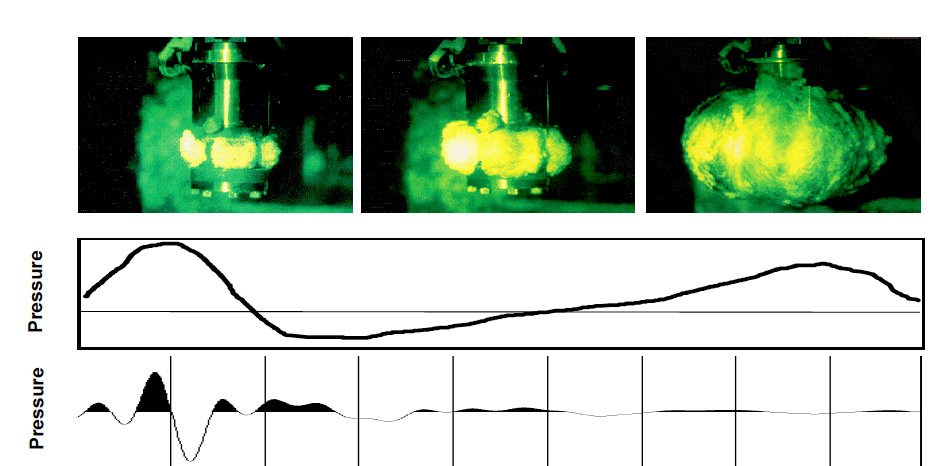
\includegraphics[width=0.8\textwidth]{Fig/airgun1.png}
  \caption{Firing of airgun}
  \label{fig:airgun1}
\end{figure}
\end{frame}
%------------------------------------------------
\begin{frame}{Marine seismic data acquisition}
%------------------------------------------------
\begin{figure}
  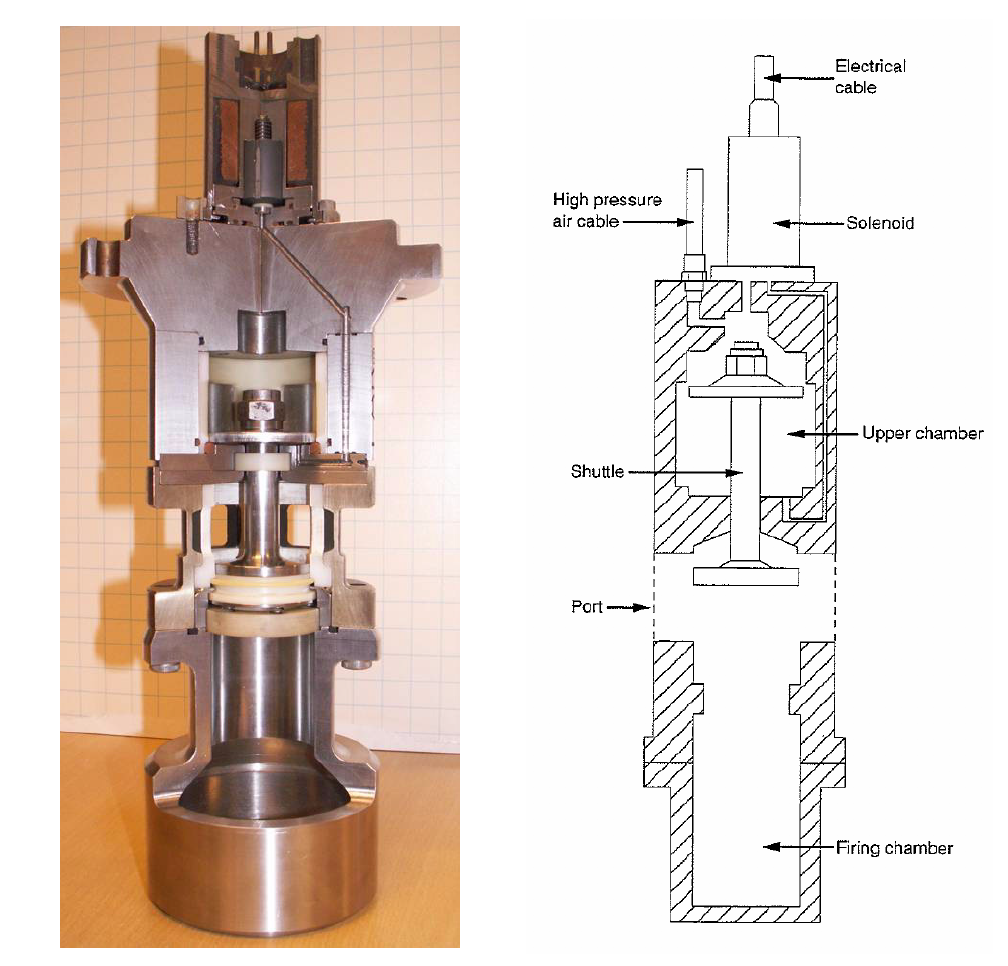
\includegraphics[width=0.6\textwidth]{Fig/airgun2.png}
  \caption{Airgun design}
  \label{fig:airgun2}
\end{figure}
\end{frame}
%-------------------------------------------------
\begin{frame}{Motion of expanding water bubble}
%-------------------------------------------------
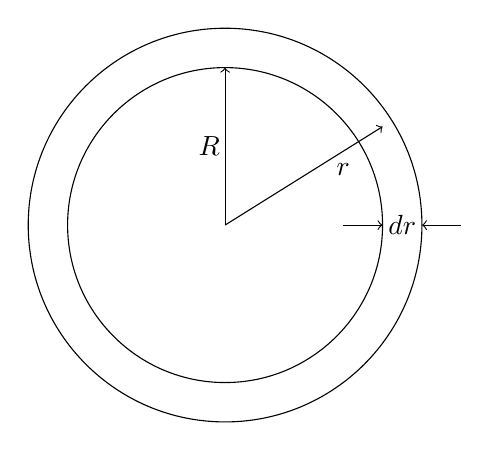
\begin{tikzpicture}
    \draw (0,0) circle [radius=2cm];
    \draw (0,0) circle [radius=2.5cm];
    \draw[->] (0,0) -- (0,2cm);
    \node[align=left] at (-0.2cm ,1cm) {$R$}; 
    \draw[->] (0,0) -- (2cm,1.25cm);
    \node at (1.5cm,0.7cm) {$r$}; 
    \draw[->] (1.5cm,0) -- (2cm,0);
    \draw[<-] (2.5cm,0) -- (3cm,0);
    \node[align=right] at (2.25cm,0) {$dr$}; 
\end{tikzpicture}
\begin{itemize}
\item $R$: Bubble wall radius
\item $U=\frac{dR}{dt}$: Bubble wall velocity
\item $r$: Water particle radius
\item $u=\frac{dr}{dt}$: Water particle velocity
\end{itemize}
\end{frame}
%------------------------------------------------
\begin{frame}{Motion of expanding water bubble}
%------------------------------------------------
The kinetic energy of a spherical shell with water with
thickness $dr$ and mass $m$ is
\begin{eqnarray}
   \frac{1}{2}m u^2 = \frac{1}{2}\rho 4\pi r^2 dr u^2
\end{eqnarray}
where $u$ is the velocity of a water particel at distance $r$.
The velocity of the surface of the shell (bubble wall) moves at
speed $U$ and has distance $R$.

The amount of mass per time unit moving accross the surface of the shell
must be constant (no mass is lost) so we must have
\begin{eqnarray}
\rho 4\pi R^2 \frac{dR}{dt} = \rho 4\pi r^2 \frac{dr}{dt},
\end{eqnarray}
or
\begin{eqnarray}
 R^2 U = r^2 u, 
\end{eqnarray}
and
\begin{eqnarray}
u = \frac{UR^2}{r^2}.
        \label{eq:u}
\end{eqnarray}
\end{frame}
%------------------------------------------------
\begin{frame}{Motion of expanding water bubble}
%------------------------------------------------
The total kinetic energi of the water motion is
(assuming the buble expands freely to infinity)
\begin{eqnarray}
E_k =\int_R^{\infty} \frac{1}{2}mu^2. 
\end{eqnarray}
using $m = \rho dV = \rho 4\pi r^2 dr$
and equation \eqref{eq:u}, I get
\begin{eqnarray}
E_k =\int_R^{\infty} 2\pi\rho U^2R^4\int_R^{\infty}\frac{dr}{r^2} 
    =2\pi\rho U^2 R^3.
\end{eqnarray}
\end{frame}
%------------------------------------------------
\begin{frame}{Motion of expanding water bubble}
%------------------------------------------------
The potential energy of the bubble with radius $R$ is
\begin{eqnarray}
E_p = \frac{4}{3}\pi (p-p_{\infty}) R^3
\end{eqnarray}
Here the pressure is $p$ and $p_{\infty}$ is
the hydrostatic pressure.
$R$ changes with time, so we are interested in
the change in potential energy from an initial position
$R_0$ to a later position $R$
\begin{eqnarray}
W = \frac{4}{3}\pi (p_0-p_{\infty}) R_0^3-\frac{4}{3}\pi (p-p_{\infty}) R^3
\end{eqnarray}
$p_0$ is the initial pressure (assumed constant in space, but not time).
The total energy is now
\begin{eqnarray}
E = E_k + W = 2\pi\rho \dot{R}^2 R^3 + 
    \frac{4}{3}\pi (p_0-p_{\infty}) R_0^3-\frac{4}{3}\pi (p-p_{\infty}) R^3.
\end{eqnarray}
where we use $U=\dot{R}$.
\end{frame}
%------------------------------------------------
\begin{frame}{Motion of expanding water bubble}
%------------------------------------------------
Since the energy is conserved, differentiating this equation 
with respect to time gives
\begin{eqnarray}
0 = 2\pi\rho \left(2\dot{R}\ddot{R}R^3 + \dot{R}^2 3R^2\dot{R}\right)
    -\frac{4}{3}\pi (p-p_{\infty}) 3R^2\dot{R} 
\end{eqnarray}
which gives Rayleigh's equation for the bubble motion
\begin{eqnarray}
  \ddot{R} R + \frac{3\dot{R}^2}{2} = \frac{(p-p_{\infty})}{\rho}
\end{eqnarray}
\end{frame}
%------------------------------------------------
\begin{frame}{Motion of expanding water bubble}
%------------------------------------------------
\begin{figure}
  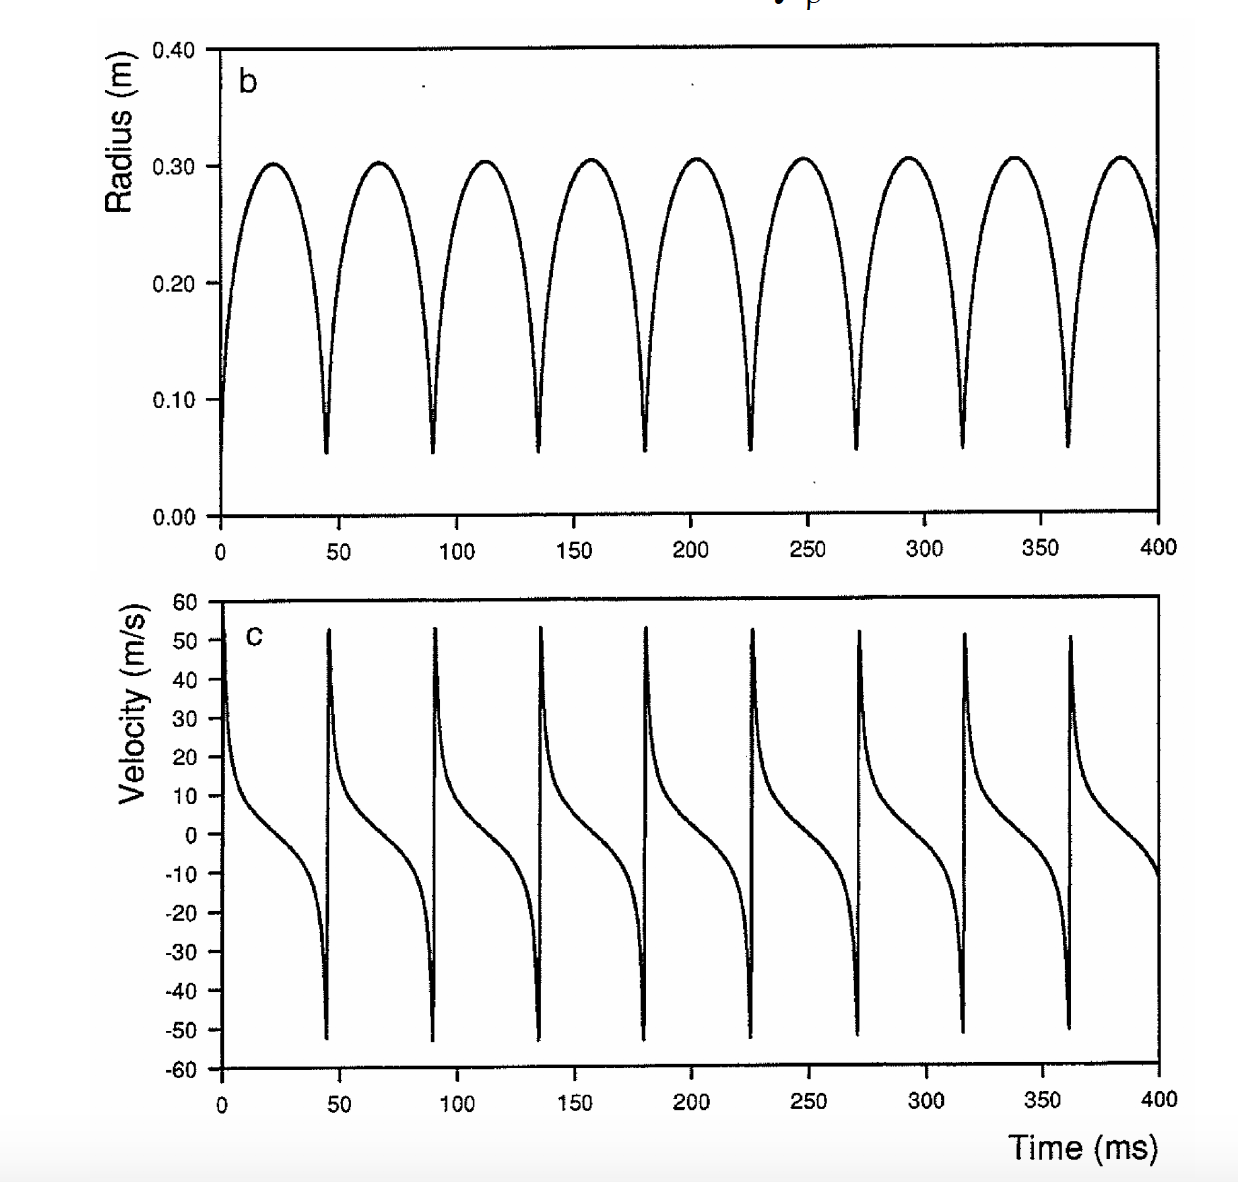
\includegraphics[width=0.6\textwidth]{Fig/rayleigh.png}
  \caption{Solution of Rayleigh's water bubble equation for
           an initial volume of 40 $\mbox{inch}^3$, firing pressure 140 bar and
            water depth 7.5 m}
  \label{fig:rayleigh}
\end{figure}
\end{frame}
%------------------------------------------------
\begin{frame}{Airgun signature}
%------------------------------------------------
The Rayleigh equation must be modified to 
model a realistic airgun. A better equation was develope by
Bethe and Kirkwood.
\begin{figure}
  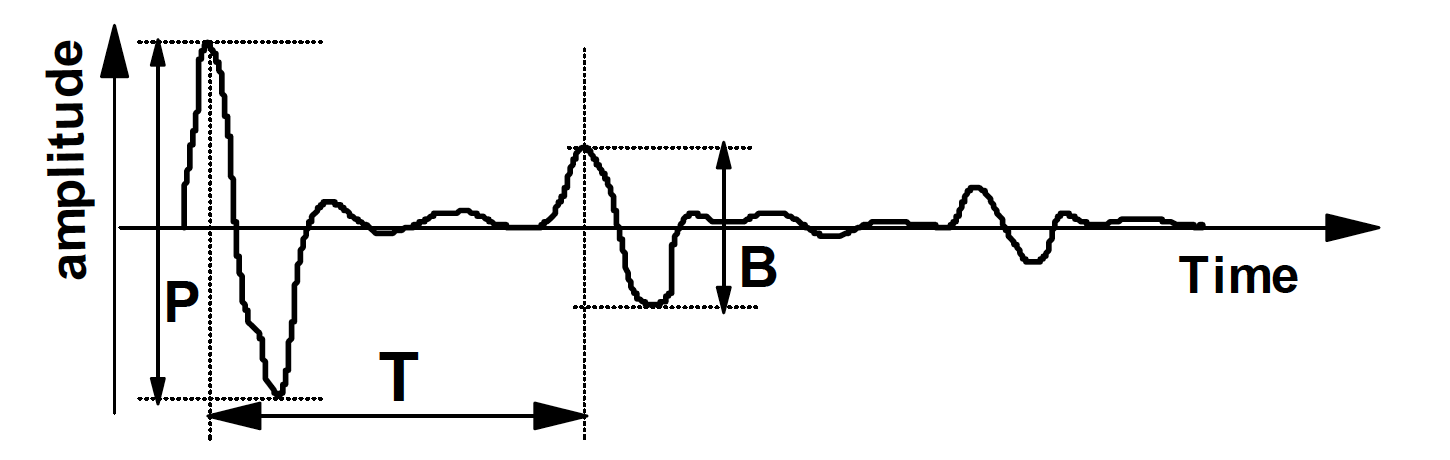
\includegraphics[width=\textwidth]{Fig/source.png}
  \caption{Measured airgun pressure, with definition
           of bubble period (T), primary peak amplitude (P)
           and bubble amplitude.}
  \label{fig:rayleigh2}
\end{figure}
\end{frame}
%------------------------------------------------
\begin{frame}{Airgun signature}
%------------------------------------------------
\begin{itemize}
\item  Primar to Bubble ratio = P/B
\item  P/B should be as large as possible
\item  Most important method fo achieve high P/B is
       clustering of airguns close together.
\item  Another approach is combining airguns with different 
       volumes
\end{itemize}
\end{frame}
%------------------------------------------------
\begin{frame}{Source signature estimation}
%------------------------------------------------
\begin{figure}
  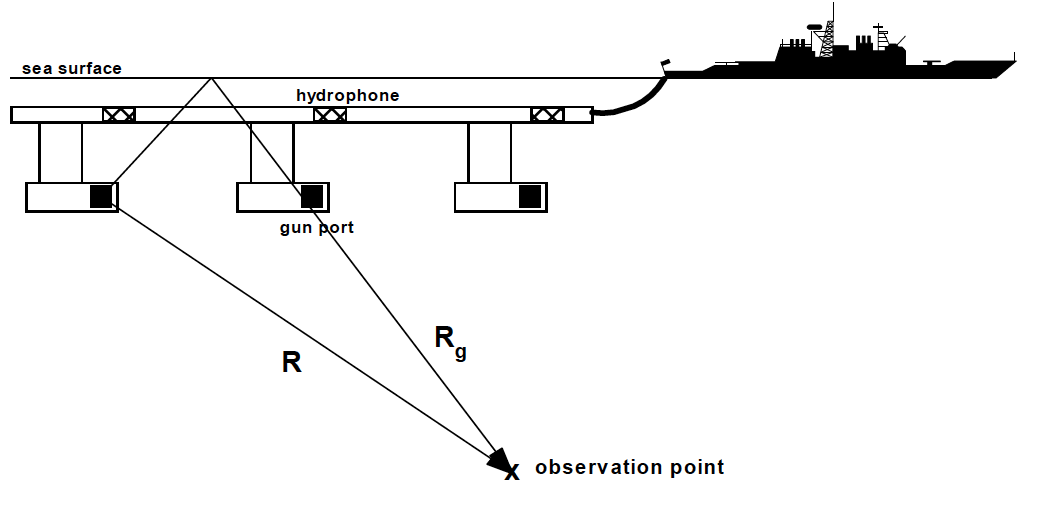
\includegraphics[width=\textwidth]{Fig/notional.png}
  \caption{Notional source measurement}
  \label{fig:notional}
\end{figure}
\end{frame}
%------------------------------------------------
\begin{frame}{Notional source method}
%------------------------------------------------
\begin{eqnarray}
    p(R,t) = \sum_j \left[\frac{S_j(t-R_j/c)}{R_j} 
                   - \frac{S_j(t-R^g_j/c)}{R^g_j}\right].
\end{eqnarray}
\begin{itemize}
\item $R_j$: Distance from source to observation point for source no $j$.
\item $R^g_j$: Distance via sea surface to observation point for source no $j$.
\item $S_j$: Notional source measurement for source no $j$.
\end{itemize}
\end{frame}
%------------------------------------------------
\begin{frame}{The source ghost spectrum}
%------------------------------------------------
\begin{figure}
  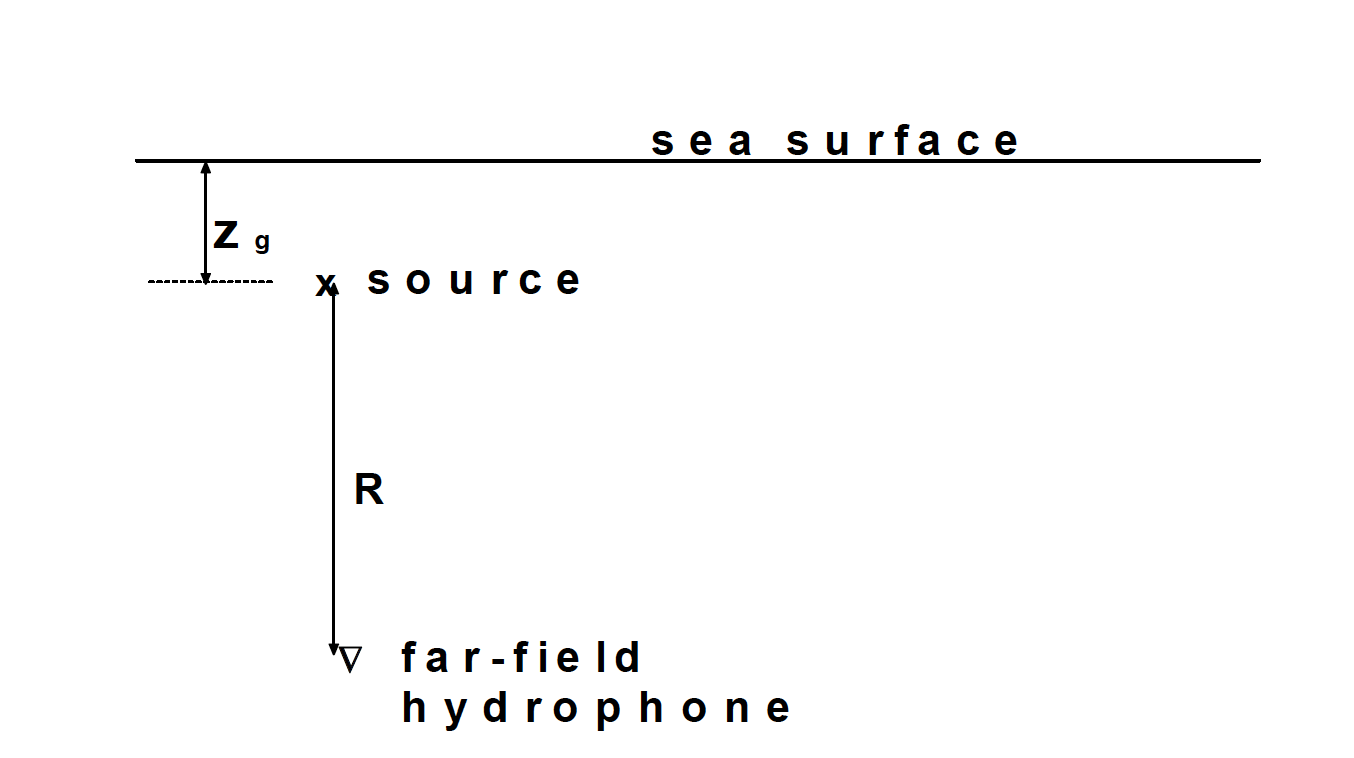
\includegraphics[width=\textwidth]{Fig/ghost.png}
  \caption{Ghost measurement setup}
  \label{fig:ghost}
\end{figure}
\end{frame}
%------------------------------------------------
\begin{frame}{The source ghost spectrum}
%------------------------------------------------
The signal measured at the far-field hydrophone is
\begin{eqnarray}
s(t) = \frac{1}{R}p(t-R/c) - \frac{1}{R_g}p(t-R_g/c)
                                \label{eq:signature-ghost}
\end{eqnarray}
here $R_g = R + 2z_g$.
The Fourier transform is defined by
\begin{eqnarray}
 S(\omega) = \int_{-\infty}^{+\infty} dt\, s(t)\exp(-i\omega t),
\end{eqnarray}
and $\omega =2\pi f$.
Fourier transforming equation \eqref{eq:signature-ghost} one gets
\begin{eqnarray}
S(\omega) = 
  \frac{1}{R}P(\omega)\exp(-i\omega R/c) 
 - \frac{1}{R_g}P(\omega)\exp(-i\omega R_g/c).
\end{eqnarray}
This is approximately ($R\approx R_g$ in the denominator)
\begin{eqnarray}
S(\omega) = 
  \frac{1}{R}P(\omega)\left[1-exp(-i2\omega z_g/c)\right]\exp(-i\omega R/c) 
\end{eqnarray}
\end{frame}
%------------------------------------------------
\begin{frame}{The source ghost spectrum}
%------------------------------------------------
\begin{eqnarray}
S(\omega) = 
  \frac{1}{R}P(\omega)\exp(-i\omega R/c) \left[1-exp(-i2\omega z_g/c)\right] 
   = \frac{1}{R}P(\omega)H(\omega).
\end{eqnarray}
$P(\omega)$ is the Fourier transform of the airgun source signal and the exponential factor is a time delay,  but
the extra factor
\begin{eqnarray}
  H(\omega)=\left[1-exp(-i2\omega z_g/c)\right], 
\end{eqnarray}
is only due to the influence of the sea surface and
describes the so-called ghost-effect.

$H$ can be written in a slightly different way
\begin{eqnarray}
S(\omega) = 
  H(\omega)=\exp(-i\omega z_g/c)
           \left[\exp(i\omega z_g/c)-exp(-i\omega z_g/c)\right].
\end{eqnarray}
\end{frame}
%------------------------------------------------
\begin{frame}{The source ghost spectrum}
%------------------------------------------------
Using the fact that $2i\sin(x) = \exp(ix)-\exp(-ix)$
we can write $H$ in the form
\begin{eqnarray}
S(\omega) = 
  H(\omega)=2i\exp(-i\omega z_g/c)\sin(\omega z_g/c)
\end{eqnarray}

The amplitude spectrum of the ghost filter $H$ can be computed by
\begin{eqnarray}
|H(\omega)|^2 = H^*(\omega)H(\omega),
\end{eqnarray}
where the * denotes complex conjugation ($i \rightarrow -i$).
We get
\begin{eqnarray}
|H(\omega)|^2 = (-2i)\exp(i\omega z_g/c)\sin(\omega z_g/c)
                2i\exp(-i\omega z_g/c)\sin(\omega z_g/c)
\end{eqnarray}
\begin{eqnarray}
|H(\omega)|^2 = 4\sin^2(\omega z_g/c)
\end{eqnarray}
\begin{eqnarray}
H(\omega) = 2|\sin(2\pi f z_g/c)|
\end{eqnarray}
\end{frame}
%------------------------------------------------
\begin{frame}{The source ghost spectrum}
%------------------------------------------------
\begin{figure}
  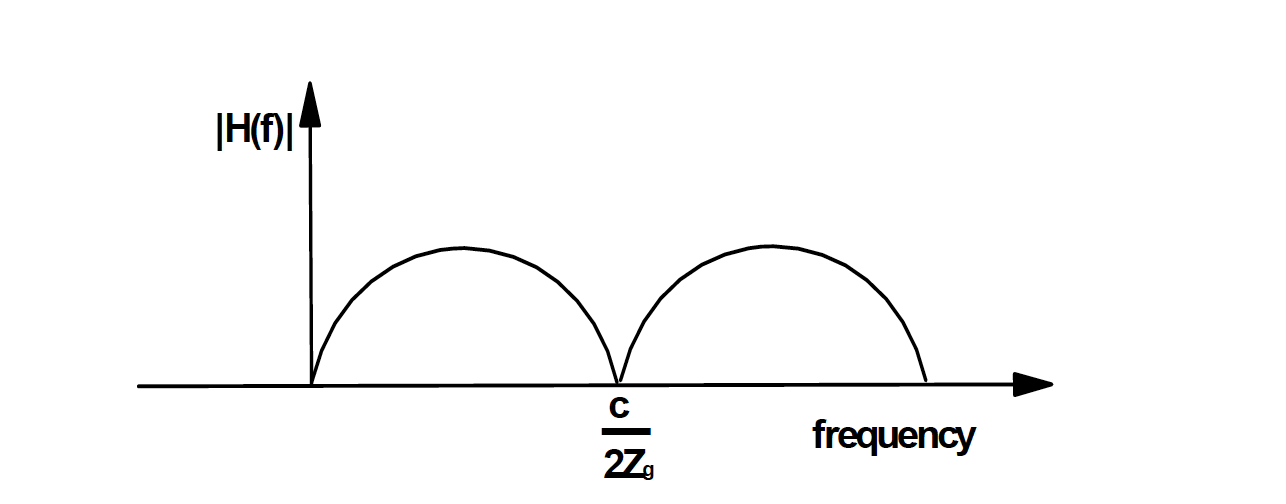
\includegraphics[width=\textwidth]{Fig/ghost-spec.png}
  \caption{Ghost filter}
  \label{fig:ghost-spec}
\end{figure}
\end{frame}
%------------------------------------------------
\begin{frame}{The source ghost spectrum}
%------------------------------------------------
\begin{figure}
  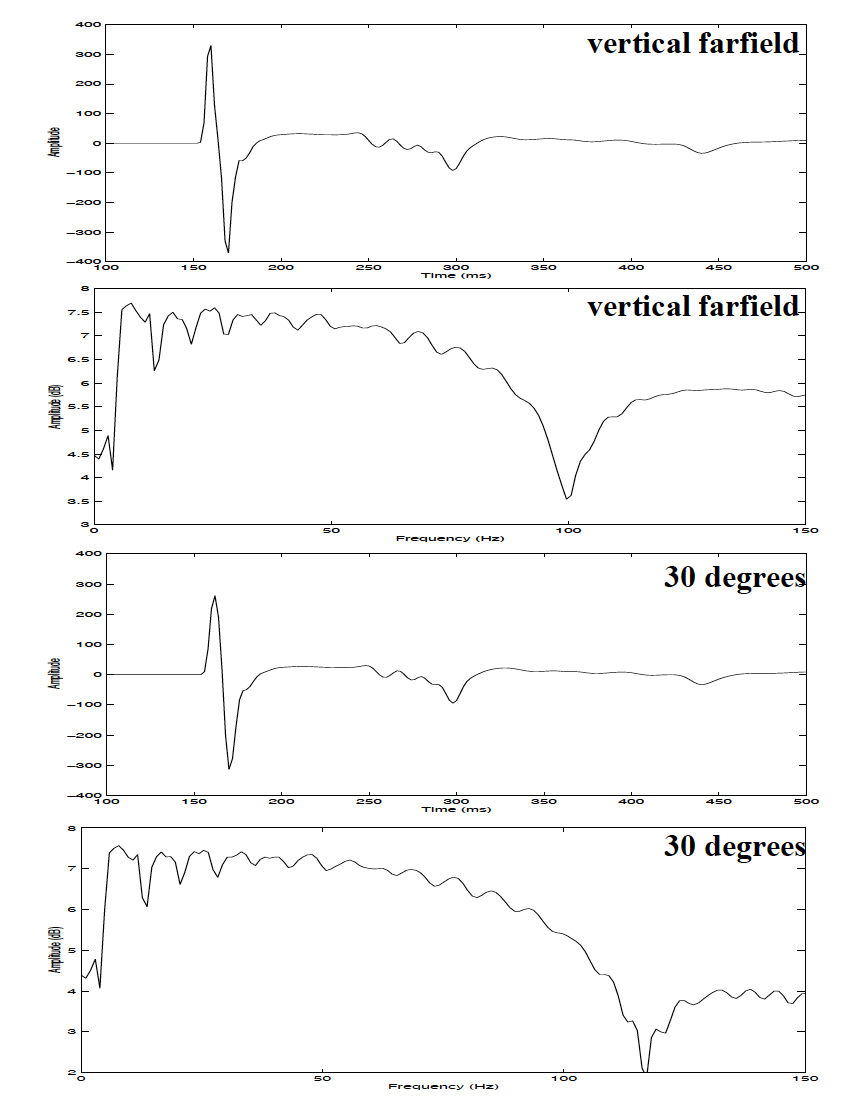
\includegraphics[width=0.5\textwidth]{Fig/ghost2.png}
  \caption{Ghost filter}
  \label{fig:ghost2}
\end{figure}
\end{frame}
%------------------------------------------------
\begin{frame}{The source ghost spectrum}
%------------------------------------------------
\begin{figure}
  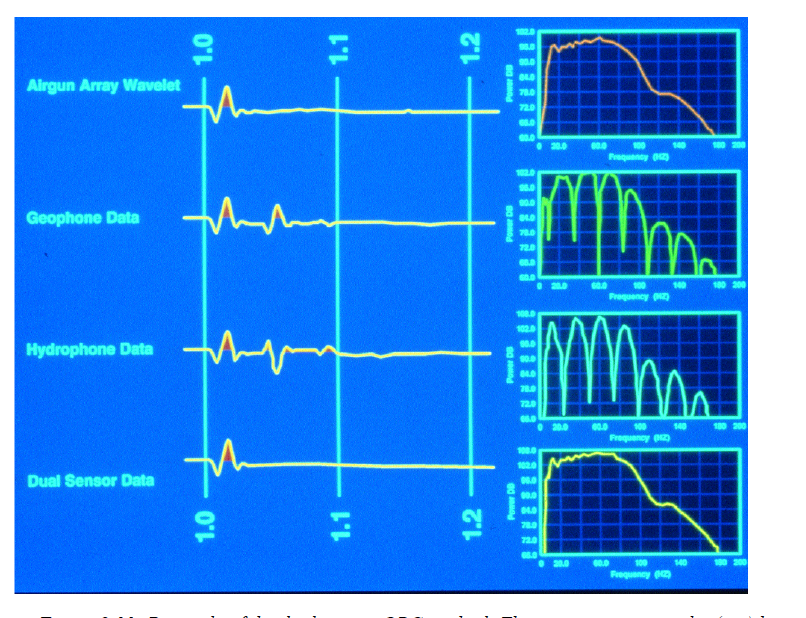
\includegraphics[width=0.8\textwidth]{Fig/ghost3.png}
  \caption{Ghost filter}
  \label{fig:ghost3}
\end{figure}
\end{frame}
\end{document}

